
%%%%%%%%%%%%%%%%%%%%%%% file typeinst.tex %%%%%%%%%%%%%%%%%%%%%%%%%
%
% This is the LaTeX source for the instructions to authors using
% the LaTeX document class 'llncs.cls' for contributions to
% the Lecture Notes in Computer Sciences series.
% http://www.springer.com/lncs       Springer Heidelberg 2006/05/04
%
% It may be used as a template for your own input - copy it
% to a new file with a new name and use it as the basis
% for your article.
%
% NB: the document class 'llncs' has its own and detailed documentation, see
% ftp://ftp.springer.de/data/pubftp/pub/tex/latex/llncs/latex2e/llncsdoc.pdf
%
%%%%%%%%%%%%%%%%%%%%%%%%%%%%%%%%%%%%%%%%%%%%%%%%%%%%%%%%%%%%%%%%%%%


\documentclass[runningheads,a4paper]{llncs}

\usepackage{multirow}
\usepackage{amsfonts}
\usepackage{array,color}
\usepackage{amsmath}
\usepackage{amssymb}
\setcounter{tocdepth}{3}
\usepackage{graphicx,floatrow}
\floatsetup[table]{capposition=top}

\usepackage{url}
\urldef{\mailsa}\path|{yu-zhao, gaosheng, lijuncen, guojun}@bupt.edu.cn|
\newcommand{\keywords}[1]{\par\addvspace\baselineskip
\noindent\keywordname\enspace\ignorespaces#1}

\begin{document}

\mainmatter  % start of an individual contribution

% first the title is needed
\title{Research of 230MHZ Radio Propagation Models}



% the name(s) of the author(s) follow(s) next
%
% NB: Chinese authors should write their first names(s) in front of
% their surnames. This ensures that the names appear correctly in
% the running heads and the author index.
%
\author{Ying,Wang \and Bo,Li \and Jianming,Zhang }
\institute{Power Grid Control Center of Guangdong, Guangzhou 510600, China\and Beijing University of Posts and Telecommunications, China\\
}

\maketitle


\begin{abstract}
Any communication system, the channel is an integral part. Channel by channel transmission medium is divided into wired and wireless channels. Performance of the wireless communication system depends largely on the radio channel. Because of the speed of electromagnetic waves by reflection, diffraction, scattering, multipath propagation and a mobile station in a wireless channel, the impact of factors such as the transmission bandwidth of the signal, so unlike the cable channel radio channel as fixed and predictable, but has a lot randomness, analysis difficult. Thus, wireless channel modeling has always been a wireless communication system research difficult. The propagation characteristics of the radio channel wireless network for the study, planning and design, has a very important role. Propagation characteristics of the radio channel, need to clear the propagation of radio channels and a variety of physical phenomena. In order to plan and provide the basis for design of communication systems, often summary and statistical analysis to establish the universality of the mathematical model or measured by theoretical analysis. Using these models, some propagation environment can be estimated propagation loss and other relevant propagation parameters, depending on the environment in the selection of different mathematical models. Thus, in different situations using appropriate mathematical model becomes very important. Propagation models need to consider various factors terrain, the type of environment and material environment, etc. It is even more important, especially in the wireless communication in mobile communications. In a wireless communication system, often through various irregular wave propagation area. In estimating the path loss, to consider topography specific areas, including simple curve shape and mountainous terrain. While also considering the impact of trees, buildings and other obstructions and other factors. In a wireless mobile communication network engineering design of wireless systems, often using a radio wave propagation loss prediction model to calculate the propagation loss of the radio path, determines that the wireless cell service coverage area.}
\end{abstract}


\section{Introduction}
\subsection{Propagation model classification}

Empirical model is reflected in a large number of wireless path through statistical analysis of the test results obtained by loss formula. Such as: Okumura-Hata, Cost231-Hata, LEE model\cite{dd}. 
Semi-empirical or semi-deterministic method to determine the mode is to be used for general urban or indoor environments derived formula. According to the experimental results can also be corrected for the equation to obtain the surrounding area function characterization of antennas specified characteristics. Such as: COST Walfish-Ikegami like. 
Deterministic model is a method for site-specific environmental applications of electromagnetic theory calculations. In this mode, several techniques have been used are usually based on electromagnetic ray tracing method - GTD (GTD)\cite{ee}, physical optics (PO) and the like. In this mode, the wireless communication and environmental characteristics (such as height of buildings, corners, street width, surface materials, etc.). 
Into the free space propagation model and non-free-space propagation model based on different mobile radio propagation environment. 
The free space is the ideal space filled with a homogeneous medium, but also affect the ground and obstacles do not exist. In the free space wave propagation does not produce reflection, refraction, scattering, diffraction and absorption phenomena, there is only the attenuation caused by diffusion. Free-space basic transmission loss refers to the transmission system located in free space equivalent isotropic radiated power (EIRP) and receiving system isotropic receiving antenna\cite{cs02} receives power ratio available in the actual system only in the range of visibility only the free space propagation model may be used between the lower transmit and receive.

\subsection{230MHZ propagation model application}

230MHZ propagation model has a number of applications, particularly in the power direction\cite{bb}. Power wireless broadband communication system used 230 MHz band dedicated power load control as a working band, TD-LTE technology will be applied to the power of wireless broadband communication systems, carrier aggregation technology polymerized by the discrete spectrum, broadband transmission; based on soft frequency reuse using technology to achieve the same frequency networking; end to end encryption system to ensure the safety of multiple security of data transmission. Developed a distributed architecture based access network equipment, core network equipment and high stability small, modular communications terminal products, and the formation of related equipment interface specifications and test specifications. Compared with the traditional public communications system, which information transfer speed, real strong\cite{cc}, stable and reliable performance, but also to support the stability of the image transmission, smart grid can meet a variety of business needs. The system is stable after a long run, for the new smart electricity business information with reliable, stable transmission provides wireless broadband channel, for the advanced wireless communication technology for smart grid construction to provide a good role model.

\section{FORMULATION OF THE 230MHZ PROPAGATION}
\label{sec:exp}

Here is the formula for calculating the propagation model of 230MHZ sub-module.

\begin{figure*}
\centerline{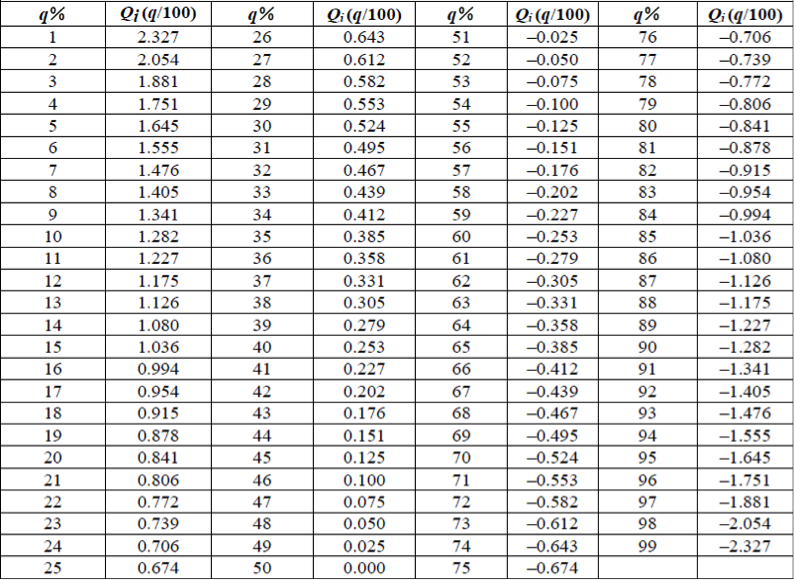
\includegraphics[width=15cm]{sheet.png}}
\caption{This is the sheet of some indicates used in the following formula.}
\label{f:fralfamap}
\end{figure*}

\subsection{The maximum free space field strength calculation method}

The maximum free space field strength calculation method is as formula blow
: \begin{equation}
{E_{\max }} = 106.9 - 20\lg (d), \label{keurough} \end{equation} where
${E_{\max }} $is the effective radiated power free-field strength,$d$ is the distance,unit is km.

\subsection{Effective height $h1$ of the transmitting antennas is determined}

 \begin{equation}
[\begin{array}{l}
{h_1} = {h_a}{\kern 1pt} {\kern 1pt} {\kern 1pt} {\kern 1pt} {\kern 1pt} {\kern 1pt} {\kern 1pt} {\kern 1pt} {\kern 1pt} {\kern 1pt} {\kern 1pt} {\kern 1pt} {\kern 1pt} {\kern 1pt} {\kern 1pt} {\kern 1pt} {\kern 1pt} {\kern 1pt} {\kern 1pt} {\kern 1pt} {\kern 1pt} {\kern 1pt} {\kern 1pt} {\kern 1pt} {\kern 1pt} {\kern 1pt} {\kern 1pt} {\kern 1pt} {\kern 1pt} {\kern 1pt} {\kern 1pt} {\kern 1pt} {\kern 1pt} {\kern 1pt} {\kern 1pt} {\kern 1pt} {\kern 1pt} {\kern 1pt} {\kern 1pt} {\kern 1pt} {\kern 1pt} {\kern 1pt} {\kern 1pt} {\kern 1pt} {\kern 1pt} {\kern 1pt} {\kern 1pt} {\kern 1pt} {\kern 1pt} {\kern 1pt} {\kern 1pt} {\kern 1pt} {\kern 1pt} {\kern 1pt} {\kern 1pt} {\kern 1pt} {\kern 1pt} {\kern 1pt} {\kern 1pt} {\kern 1pt} {\kern 1pt} {\kern 1pt} {\kern 1pt} {\kern 1pt} {\kern 1pt} {\kern 1pt} {\kern 1pt} {\kern 1pt} {\kern 1pt} {\kern 1pt} {\kern 1pt} {\kern 1pt} {\kern 1pt} {\kern 1pt} {\kern 1pt} {\kern 1pt} {\kern 1pt} {\kern 1pt} {\kern 1pt} {\kern 1pt} {\kern 1pt} {\kern 1pt} {\kern 1pt} {\kern 1pt} {\kern 1pt} {\kern 1pt} {\kern 1pt} {\kern 1pt} {\kern 1pt} {\kern 1pt} {\kern 1pt} {\kern 1pt} {\kern 1pt} {\kern 1pt} {\kern 1pt} {\kern 1pt} {\kern 1pt} {\kern 1pt} {\kern 1pt} {\kern 1pt} {\kern 1pt} {\kern 1pt} {\kern 1pt} {\kern 1pt} {\kern 1pt} {\kern 1pt} {\kern 1pt} {\kern 1pt} {\kern 1pt} {\kern 1pt} {\kern 1pt} {\kern 1pt} {\kern 1pt} {\kern 1pt} {\kern 1pt} {\kern 1pt} {\kern 1pt} {\kern 1pt} {\kern 1pt} {\kern 1pt} {\kern 1pt} {\kern 1pt} {\kern 1pt} {\kern 1pt} {\kern 1pt} {\kern 1pt} {\kern 1pt} {\kern 1pt} {\kern 1pt} {\kern 1pt} {\kern 1pt} {\kern 1pt} {\kern 1pt} {\kern 1pt} {\kern 1pt} {\kern 1pt} {\kern 1pt} {\kern 1pt} {\kern 1pt} {\kern 1pt} {\kern 1pt} {\kern 1pt} {\kern 1pt} {\kern 1pt} {\kern 1pt} {\kern 1pt} (d \le 3km)\\
{h_1} = {h_a} + \frac{{({h_{eff}} - {h_a})(d - 3)}}{{12}}{\kern 1pt} {\kern 1pt} {\kern 1pt} {\kern 1pt} {\kern 1pt} {\kern 1pt} {\kern 1pt} {\kern 1pt} {\kern 1pt} {\kern 1pt} {\kern 1pt} {\kern 1pt} {\kern 1pt} {\kern 1pt} {\kern 1pt} {\kern 1pt} {\kern 1pt} {\kern 1pt} {\kern 1pt} {\kern 1pt} {\kern 1pt} {\kern 1pt} {\kern 1pt} {\kern 1pt} {\kern 1pt} {\kern 1pt} {\kern 1pt} {\kern 1pt} {\kern 1pt} {\kern 1pt} {\kern 1pt} {\kern 1pt} {\kern 1pt} {\kern 1pt} {\kern 1pt} {\kern 1pt} {\kern 1pt} {\kern 1pt} {\kern 1pt} {\kern 1pt} {\kern 1pt} {\kern 1pt} {\kern 1pt} {\kern 1pt} {\kern 1pt} {\kern 1pt} {\kern 1pt} {\kern 1pt} {\kern 1pt} {\kern 1pt} {\kern 1pt} {\kern 1pt} (3km < d \le 15km)\\
{h_1} = {h_{eff}}{\kern 1pt} {\kern 1pt} {\kern 1pt} {\kern 1pt} {\kern 1pt} {\kern 1pt} {\kern 1pt} {\kern 1pt} {\kern 1pt} {\kern 1pt} {\kern 1pt} {\kern 1pt} {\kern 1pt} {\kern 1pt} {\kern 1pt} {\kern 1pt} {\kern 1pt} {\kern 1pt} {\kern 1pt} {\kern 1pt} {\kern 1pt} {\kern 1pt} {\kern 1pt} {\kern 1pt} {\kern 1pt} {\kern 1pt} {\kern 1pt} {\kern 1pt} {\kern 1pt} {\kern 1pt} {\kern 1pt} {\kern 1pt} {\kern 1pt} {\kern 1pt} {\kern 1pt} {\kern 1pt} {\kern 1pt} {\kern 1pt} {\kern 1pt} {\kern 1pt} {\kern 1pt} {\kern 1pt} {\kern 1pt} {\kern 1pt} {\kern 1pt} {\kern 1pt} {\kern 1pt} {\kern 1pt} {\kern 1pt} {\kern 1pt} {\kern 1pt} {\kern 1pt} {\kern 1pt} {\kern 1pt} {\kern 1pt} {\kern 1pt} {\kern 1pt} {\kern 1pt} {\kern 1pt} {\kern 1pt} {\kern 1pt} {\kern 1pt} {\kern 1pt} {\kern 1pt} {\kern 1pt} {\kern 1pt} {\kern 1pt} {\kern 1pt} {\kern 1pt} {\kern 1pt} {\kern 1pt} {\kern 1pt} {\kern 1pt} {\kern 1pt} {\kern 1pt} {\kern 1pt} {\kern 1pt} {\kern 1pt} {\kern 1pt} {\kern 1pt} {\kern 1pt} {\kern 1pt} {\kern 1pt} {\kern 1pt} {\kern 1pt} {\kern 1pt} {\kern 1pt} {\kern 1pt} {\kern 1pt} {\kern 1pt} {\kern 1pt} {\kern 1pt} {\kern 1pt} {\kern 1pt} {\kern 1pt} {\kern 1pt} {\kern 1pt} {\kern 1pt} {\kern 1pt} {\kern 1pt} {\kern 1pt} {\kern 1pt} {\kern 1pt} {\kern 1pt} {\kern 1pt} {\kern 1pt} {\kern 1pt} {\kern 1pt} {\kern 1pt} {\kern 1pt} {\kern 1pt} {\kern 1pt} {\kern 1pt} {\kern 1pt} {\kern 1pt} {\kern 1pt} {\kern 1pt} {\kern 1pt} {\kern 1pt} {\kern 1pt} {\kern 1pt} {\kern 1pt} {\kern 1pt} {\kern 1pt} {\kern 1pt} {\kern 1pt} {\kern 1pt} {\kern 1pt} {\kern 1pt} {\kern 1pt} {\kern 1pt} {\kern 1pt} {\kern 1pt} {\kern 1pt} {\kern 1pt} {\kern 1pt} {\kern 1pt} {\kern 1pt} {\kern 1pt} {\kern 1pt} {\kern 1pt} {\kern 1pt} (d > 15km)
\end{array}, \label{keurough} \end{equation} 

Here, the height of the antenna above the ground. the actual height of the antenna unit is $m$; between the transmitting antenna to the mobile station antenna, the direction of 3-15 $km$ from the ground exceeds the average height of the antenna, the unit is $m$; $d$ is the distance from the base station to the user between units of $km$.

\subsection{Correction of the frequency $f$}

We could check the sheet to find the value of $E_{inf}$ and ${E_{sup}$, then we can use the formula to get the value of field intensity $E$

\begin{equation}
E = {E_{inf}} + ({E_{sup}} - {E_{inf}})\frac{{lg(\frac{f}{{{f_{inf}}}})}}{{\lg (\frac{{{f_{sup}}}}{{{f_{inf}}}})}}, \label{keurough} \end{equation}

\subsection{Correction of the percentage of time $t$}

For the time $t$ required to make a percentage of the value of the field strength can be derived as follows:

\begin{equation}
E = {E_{sup}}\frac{{({Q_{inf}} - {Q_t})}}{{({Q_{inf}} - {Q_{sup}})}} + {E_{inf}}\frac{{({Q_t} - {Q_{sup}})}}{{({Q_{inf}} - {Q_{sup}})}}, \label{keurough} \end{equation}

\subsection{Shot path correct}

If the length is shorter than 15 km in the path of the flat terrain buildings comprising a plurality of uniform height\cite{cr05}, the field should be added to the field strength due to the construction to reduce the clutter caused by the strong correction amount. That is, when d is less than 15 km and when h1-R is less than 150 m, the field strength value should be added to the following corrections:

\begin{equation}
C =  - 3.3[lg(f)][1 - 0.85lg(d)][1 - 0.46lg(1 + {h_a} - R)], \label{keurough} \end{equation}

Where in, ${h_a}$ height of the antenna above the ground (m) (i.e., the height of the mast), $R$ in the reception of the earth around the antenna height of the coating, it also represents the transmit antenna of the earth around the coating height.

\subsection{Correction of the percentage of time $t$}

For the time $t$ required to make a percentage of the value of the field strength can be derived as follows:

\begin{equation}
E = {E_{sup}}\frac{{({Q_{inf}} - {Q_t})}}{{({Q_{inf}} - {Q_{sup}})}} + {E_{inf}}\frac{{({Q_t} - {Q_{sup}})}}{{({Q_{inf}} - {Q_{sup}})}}, \label{keurough} \end{equation}

Where in, ha height of the antenna above the ground (m) (i.e., the height of the mast), R in the reception of the earth around the antenna height of the coating, it also represents the transmit antenna of the earth around the coating height.


\subsection{Location variability correction}

The position of the receiving antenna on the land, the excess correction term given by the following equation q position of the point:

\begin{equation}
{C_p}(q) = {Q_i}(\frac{q}{{100}}){\sigma _L}(f)\;\;\;\;\;\;\;\;\;\;dB(\mu v/m), \label{keurough} \end{equation}


\subsection{Correcting the receiving antenna}

Field strength values by land curves and related forms given height reference value $R$(m) of the receiving antenna height $R$ (m) reflects the receiving antenna of the earth around the height of the coating, the condition for the minimum height 10 m. For example, in urban areas a reference height of 20 m, within a dense urban areas and 30 m, in the suburban area of 10 m. 
When the receiving antenna is on the ground, first taking into account the elevation angle of the radio wave arrival, by the following formula to calculate the height of the modified representation of the field scattered $R$ '(m):

\begin{equation}
{\rm{R' = }}\frac{{1000dR - 15{h_1}}}{{1000d - 15}}{\kern 1pt} {\kern 1pt} {\kern 1pt} {\kern 1pt} {\kern 1pt} {\kern 1pt} {\kern 1pt} {\kern 1pt} {\kern 1pt} {\kern 1pt} {\kern 1pt} {\kern 1pt} {\kern 1pt} {\kern 1pt} {\kern 1pt} {\kern 1pt} {\kern 1pt} {\kern 1pt} {\kern 1pt} {\kern 1pt} {\kern 1pt} {\kern 1pt} {\kern 1pt} {\kern 1pt} {\kern 1pt} {\kern 1pt} {\kern 1pt} {\kern 1pt} {\kern 1pt} {\kern 1pt} {\kern 1pt} {\kern 1pt} {\kern 1pt} {\kern 1pt} {\kern 1pt} {\kern 1pt} m, \label{keurough} \end{equation}

Wherein, $h1$ and $R$ unit is m, the distance d in units of km. Note $h1$ \leq 6.5$d$ + $R$ . 

\subsection{Correcting the distance value $d$}

Firstly, we can get the value of $d_{nf}$ according to the gain $G$ and frequency $f$ transmitting antenna:
\begin{equation}
{d_{nf}} = \frac{{{{10}^{0.1G}}}}{{10f}}(km), \label{keurough} \end{equation}

Again according to the size $d$ is calculated by the following method field strength:
\begin{equation}
\begin{array}{l}
E = {E_{maxdnf}}{\kern 1pt} {\kern 1pt} {\kern 1pt} {\kern 1pt} {\kern 1pt} {\kern 1pt} {\kern 1pt} {\kern 1pt} {\kern 1pt} {\kern 1pt} {\kern 1pt} {\kern 1pt} {\kern 1pt} {\kern 1pt} {\kern 1pt} {\kern 1pt} {\kern 1pt} {\kern 1pt} {\kern 1pt} {\kern 1pt} {\kern 1pt} {\kern 1pt} {\kern 1pt} {\kern 1pt} {\kern 1pt} {\kern 1pt} {\kern 1pt} {\kern 1pt} {\kern 1pt} {\kern 1pt} {\kern 1pt} {\kern 1pt} {\kern 1pt} {\kern 1pt} {\kern 1pt} {\kern 1pt} {\kern 1pt} {\kern 1pt} {\kern 1pt} {\kern 1pt} {\kern 1pt} {\kern 1pt} {\kern 1pt} {\kern 1pt} {\kern 1pt} {\kern 1pt} {\kern 1pt} {\kern 1pt} {\kern 1pt} {\kern 1pt} {\kern 1pt} {\kern 1pt} {\kern 1pt} {\kern 1pt} {\kern 1pt} {\kern 1pt} {\kern 1pt} {\kern 1pt} {\kern 1pt} {\kern 1pt} {\kern 1pt} {\kern 1pt} {\kern 1pt} {\kern 1pt} {\kern 1pt} {\kern 1pt} {\kern 1pt} {\kern 1pt} {\kern 1pt} {\kern 1pt} {\kern 1pt} {\kern 1pt} {\kern 1pt} {\kern 1pt} {\kern 1pt} {\kern 1pt} {\kern 1pt} {\kern 1pt} {\kern 1pt} {\kern 1pt} {\kern 1pt} {\kern 1pt} {\kern 1pt} {\kern 1pt} {\kern 1pt} {\kern 1pt} {\kern 1pt} {\kern 1pt} {\kern 1pt} {\kern 1pt} {\kern 1pt} {\kern 1pt} {\kern 1pt} {\kern 1pt} {\kern 1pt} {\kern 1pt} {\kern 1pt} {\kern 1pt} {\kern 1pt} {\kern 1pt} {\kern 1pt} {\kern 1pt} {\kern 1pt} {\kern 1pt} {\kern 1pt} {\kern 1pt} {\kern 1pt} {\kern 1pt} {\kern 1pt} {\kern 1pt} {\kern 1pt} {\kern 1pt} {\kern 1pt} {\kern 1pt} {\kern 1pt} {\kern 1pt} {\kern 1pt} {\kern 1pt} {\kern 1pt} {\kern 1pt} {\kern 1pt} {\kern 1pt} {\kern 1pt} {\kern 1pt} {\kern 1pt} {\kern 1pt} {\kern 1pt} {\kern 1pt} d < {d_{nf}}\\
E = {E_{maxd}}{\kern 1pt} {\kern 1pt} {\kern 1pt} {\kern 1pt} {\kern 1pt} {\kern 1pt} {\kern 1pt} {\kern 1pt} {\kern 1pt} {\kern 1pt} {\kern 1pt} {\kern 1pt} {\kern 1pt} {\kern 1pt} {\kern 1pt} {\kern 1pt} {\kern 1pt} {\kern 1pt} {\kern 1pt} {\kern 1pt} {\kern 1pt} {\kern 1pt} {\kern 1pt} {\kern 1pt} {\kern 1pt} {\kern 1pt} {\kern 1pt} {\kern 1pt} {\kern 1pt} {\kern 1pt} {\kern 1pt} {\kern 1pt} {\kern 1pt} {\kern 1pt} {\kern 1pt} {\kern 1pt} {\kern 1pt} {\kern 1pt} {\kern 1pt} {\kern 1pt} {\kern 1pt} {\kern 1pt} {\kern 1pt} {\kern 1pt} {\kern 1pt} {\kern 1pt} {\kern 1pt} {\kern 1pt} {\kern 1pt} {\kern 1pt} {\kern 1pt} {\kern 1pt} {\kern 1pt} {\kern 1pt} {\kern 1pt} {\kern 1pt} {\kern 1pt} {\kern 1pt} {\kern 1pt} {\kern 1pt} {\kern 1pt} {\kern 1pt} {\kern 1pt} {\kern 1pt} {\kern 1pt} {\kern 1pt} {\kern 1pt} {\kern 1pt} {\kern 1pt} {\kern 1pt} {\kern 1pt} {\kern 1pt} {\kern 1pt} {\kern 1pt} {\kern 1pt} {\kern 1pt} {\kern 1pt} {\kern 1pt} {\kern 1pt} {\kern 1pt} {\kern 1pt} {\kern 1pt} {\kern 1pt} {\kern 1pt} {\kern 1pt} {\kern 1pt} {\kern 1pt} {\kern 1pt} {\kern 1pt} {\kern 1pt} {\kern 1pt} {\kern 1pt} {\kern 1pt} {\kern 1pt} {\kern 1pt} {\kern 1pt} {\kern 1pt} {\kern 1pt} {\kern 1pt} {\kern 1pt} {\kern 1pt} {\kern 1pt} {\kern 1pt} {\kern 1pt} {\kern 1pt} {\kern 1pt} {\kern 1pt} {\kern 1pt} {\kern 1pt} {\kern 1pt} {\kern 1pt} {\kern 1pt} {\kern 1pt} {\kern 1pt} {\kern 1pt} {\kern 1pt} {\kern 1pt} {\kern 1pt} {\kern 1pt} {\kern 1pt} {\kern 1pt} {\kern 1pt} {\kern 1pt} {\kern 1pt} {\kern 1pt} {\kern 1pt} {\kern 1pt} {\kern 1pt} {\kern 1pt} {\kern 1pt} {\kern 1pt} {\kern 1pt} {\kern 1pt} {\kern 1pt} {d_{nf}} \le d < 0.1km\\
E = {E_{0.1km}} + ({E_{1km}} - {E_{0.1km}}){\kern 1pt} {\kern 1pt} {\kern 1pt} \lg (\frac{d}{{0.1}}){\kern 1pt} {\kern 1pt} {\kern 1pt} {\kern 1pt} {\kern 1pt} {\kern 1pt} {\kern 1pt} {\kern 1pt} {\kern 1pt} {\kern 1pt} {\kern 1pt} {\kern 1pt} {\kern 1pt} {\kern 1pt} {\kern 1pt} {\kern 1pt} {\kern 1pt} {\kern 1pt} {\kern 1pt} {d_{nf}} \le d < 0.1km
\end{array}, \label{keurough} \end{equation}

\begin{figure*}
\centerline{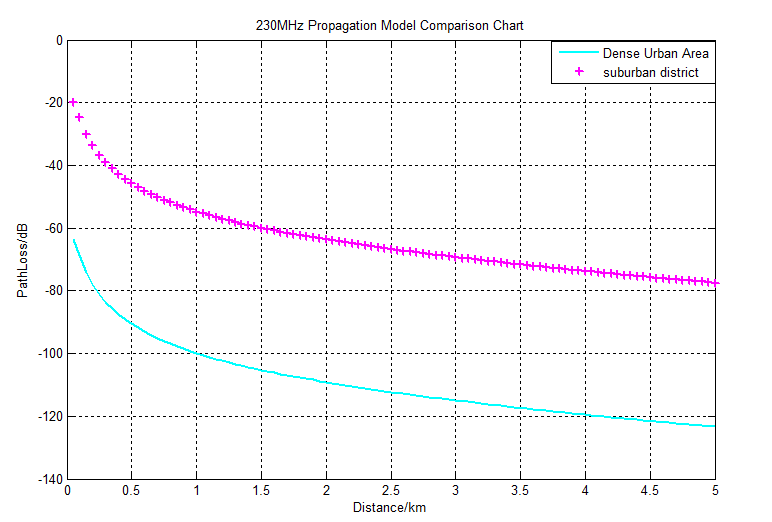
\includegraphics[width=15cm]{urbancountry.png}}
\caption{230MHZ propagation model simulation results of urban and suburban }
\end{figure*}

\begin{figure*}
\centerline{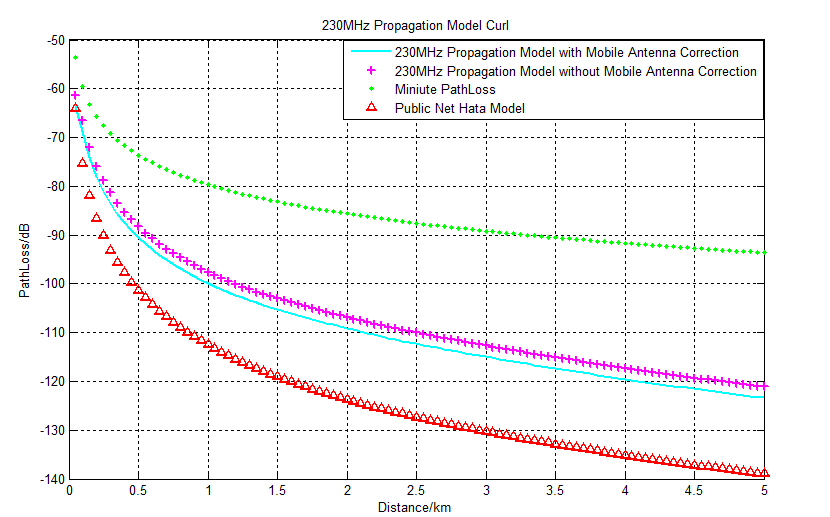
\includegraphics[width=15cm]{differentspace.png}}
\caption{Compare 230MHZ propagation model and HATA model }
\end{figure*}

\section{230MHZ PROPAGATION MODEL SIMULATION RESULTS}

In this section we see the results of the application of the principle 230MHZ in the power system. The data comes from electric communication network systems. Specific parameters are set as follows:

Percentage of time: 50\% 

Percentage Location: 50\% 

Frequency: 230$M$ 

Antenna level height: 15$m$ 

Surrounding building height: 10$m$ 

The mobile station height: 1.5$m$ 

Base Gain: 17$dbi$ 

Distance 1$km$ 

Sampling Accuracy 0.01$m$

\subsection{Correcting the receiving antenna}

The Figure2 below is Urban and suburban comparison chart. In the 230MHZ propagation models, there are significant differences between the urban and suburban ones.  We can divid this difference by correcting the reception antenna is adjusted, the height of the reception antenna rural low, and the height of the reception antenna of the city higher. For example, in urban areas a reference height of 20 m, within a dense urban areas and 30 m, in the suburban area of 10 m.

The simulation graph we can conclude that, 230MHZ propagation model in the same circumstances, the path loss will be less than the rural city. Therefore, when using 230MHZ propagation model, we should fix the propagation model according to  the different geographical conditions.


\subsection{Compare 230MHZ propagation model and HATA model}

Figure 3 is about  the comparison of 230MHZ propagation and HATA model. In the data of the power system, because some of the advantages of 230MHZ, which is less than the path loss to the path loss 1800MHZ at Hata model.





\section{CONCLUSIONS}

230MHZ compared to the public network, its low frequency, longer wavelength, long-wave transmission main deficiencies in the following areas. Surface wave attenuation due to slow wave transmitting station sent to other stations accept interference is strong. Days electrical interference on longwave acceptance severely affected, especially in summer thunderstorms more. Meanwhile, because the wavelength is longer, the requirement for higher receiving antenna, the receiving antenna needs a larger area, and the long wave receiving antenna is poor durability and maintenance costs required is relatively high.

But in LTE230 power industry Communication Network mainly for electricity distribution and transmission side of the business side needs special authorization deployed in 230MHz band power, is the depth of customization for power users wide coverage, high security, high-capacity, high-efficiency Wireless Network systems. Meanwhile, LTE230 special authorization system can be directly deployed in the 230MHz band power, in line with national policy on technical upgrading of low frequency. LTE230 systems in the power industry have major support business information collection, transmission line monitoring, distribution automation, load control, emergency videos, and other rescue headquarters. 

 LTE230 system has a wide coverage, high capacity, high security, high efficiency, high reliability, strong adaptability spectrum, deployment and expansion of smoothing and other advantages. LTE230 system work in 230MHz band, compared with the high frequency signal propagation distance farther, diffraction ability\cite{gg}. In addition, LTE230 system uses more efficient terminal transmitter technology and high sensitivity receiver technology, greatly enhance the system coverage, can achieve a wide range of high quality wireless coverage. LTE230 systems in dense urban coverage radius of up to 3 km, covering a radius of 30 kilometers to reach Kongkuo region. LTE230 system is designed to ensure that all terminals in real time online, sharing resources, data transmission terminal when the dynamic allocation of resources. Meanwhile, the signaling by streamlining processes, reducing system overhead, to ensure real-time support large terminals. Each logic cell system supports thousands of real-time online terminals. Because a single base station to accommodate an increase in the number of terminals, deployment, and construction costs are significantly reduced.  LTE230 system combines wireless applications upstream industry large amount of data, the characteristics of a small amount of data downlink, using up large resources of small asymmetric ratio of downlink mode, avoiding extensive collection applications downlink serious waste of resources problem\cite{ff}. In addition, LTE230 system uses an improved carrier aggregation, OFDM, higher order modulation (supports 64QAM) and other leading technology greatly improves wireless transmission efficiency, spectrum efficiency of the system compared to the number of transfer stations increased by several times. 
 
LTE230 system uses Turbo code and convolutional code channel encoding technology, and support for the physical layer and link layer HARQ retransmissions ARQ retransmission, good way to ensure the reliability of data transmission. In addition, the development of LTE230 system is always in scientific and standardized quality assurance system carried out by the R & D system-level evaluation CMMI5, products strictly in accordance with the national industry standard design, development, testing, final product after demanding high temperature, salt spray, vibration, lightning, dust experiments. Complete system from the fundamental guarantee for the stable and reliable products, which can cope with the complex application environment.
\bibliographystyle{chicaco}
\bibliography{typeinst}
\end{document}
